\documentclass[a4paper,11pt]{article}

\usepackage{amsmath}
\usepackage{amssymb}
\usepackage{amsthm}
\usepackage{graphicx}
\usepackage{enumerate}
\usepackage{stmaryrd}
\usepackage{setspace}
\usepackage{tikz}
\usepackage{cleveref}
\usetikzlibrary{matrix}
%you can add more packages using the same code above

%------------------

%\setlength{\topmargin}{0.0in}
%\setlength{\textheight}{10in}
%\setlength{\oddsidemargin}{0.0in}
%\setlength{\evensidemargin}{0.0in}
%\setlength{\textwidth}{6.5in}

%-------------------
\newtheorem{theorem}{Theorem}[section]
\newtheorem{proposition}[theorem]{Proposition}
\newtheorem{lemma}[theorem]{Lemma}
\newtheorem{corollary}[theorem]{Corollary}
\newtheorem{conjecture}[theorem]{Conjecture}


\theoremstyle{definition}
\newtheorem{definition}[theorem]{Definition}
\newtheorem*{example}{Example}

%------------------

%Everything before begin document is called the pre-amble and sets out how the document will look
%It is recommended you don't touch the pre-amble until you are familiar with LateX

\begin{document}

\title{Crash-Deterministic Property in Agda}
%\author{Lin Tzu Chi}
%\date{}
\maketitle

\begin{abstract}
	We have proved crash-deterministic properties in Agda.
\end{abstract}

%The following code is not run because of the percentage sign, but you might find it useful for future work
% \tableofcontents

\section{Datatypes}

To define the theorem, following datatypes(definitions) are required,
we assume that three sets are given,  
$$\mathit{Addr}, \mathit{Data}, \mathit{ProgState}$$
where $\mathit{Addr}$ is the set of all possible addresses, $\mathit{Data}$ is of all possible values, $\mathit{ProgState}$ is of all states in the program.

\begin{align*}
%\noalign{\center{\small{State of Spec, a pair of two mappings from Address to Data, representing abstracted volatile and stable states respectively.}}}
	\mathit{SpecState} ={} &(Addr \to Data) \times (Addr \to Data)\\
%\noalign{\center{\small{State of Prog, we don't have to know the details.}}}
	\mathit{ProgState^{\dagger}} ={} &\{\, \mathit{rs} \in \mathit{ProgState} \mid \mathit{RI(rs) \lor CI(rs)} \,\}\\
	\mathit{Action} ={} &\{\,\mathsf w_{addr, data} \mid addr \in Addr, data \in Data \,\} \\
	\cup \ &\{\, \mathsf {w^c}_{addr, data} \mid addr \in Addr, data \in Data \,\}\\
	\cup \ &\{ \mathsf f,\mathsf r,\mathsf {f^c},\mathsf {r^c}\}\\
	\mathit{Fragment} ={} &\mathit{Action^*}\\
\end{align*}

$\mathit{SpecState}$ is the set of all states in the operational specification, which are pairs of mappings from $Addr$ to $Data$. these two mappings represent the volatile and stable memory state of the specification. $ProgState^\dagger$ is a subset of $ProgState$ we care \---- states that satisfies either Representation Invariance or Crash Invariance. $Action$ is the set of all possible actions, and $\mathit{Fragment}$ is of all possible sequences of actions. ($^*$ is Kleene star)

And we need functions to represent actions of reading from states:
\begin{align*}
	read &: \mathit{ProgState} \to (\mathit{Addr} \to \mathit{Data})\\
	volatile &: \mathit{SpecState} \to (\mathit{Addr} \to \mathit{Data})\\
	stable &: \mathit{SpecState} \to (\mathit{Addr} \to \mathit{Data})
\end{align*}

\newpage

Single-step transitions are defined as relations on pairs of states indexed by $\mathit{Action}$, and multi-step transitions as their reflextive transitive closures (indexed by $\mathit{Fragmant}$). We assume a familiy of relations is given:
\begin{align*}
	\{ \llbracket a \rrbracket^P \subseteq \mathit{ProgState \times ProgState} \}_\mathit{a \in Action}
\end{align*}

which represents single-step transitions on $\mathit{ProgState}$,
transitions on $\mathit{SpecState}$ and $\mathit{ProgState^\dagger}$ are defined as families of relations $\{ \llbracket a \rrbracket \}_\mathit{a \in Action}$ and $\{ \llbracket a \rrbracket^\dagger \}_\mathit{a \in Action}$, with each relation defined as follows:
\begin{align*}
	\llbracket \mathsf w_{addr, data} \rrbracket ={}& \{\, (s, s') \in SpecState \times SpecState\\ &\mid \mathit{volatile(s)[addr \mapsto data]} \equiv \mathit{volatile(s')}
	\land stable(s) \equiv stable(s') \,\} \\
	\llbracket \mathsf f \rrbracket ={}& \{\, (s, s') \in SpecState \times SpecState\\ & \mid \mathit{volatile(s)} \equiv \mathit{volatile(s')} \land \mathit{volatile(s)} \equiv \mathit{stable(s')}\,\} \,\} \\
	\llbracket \mathsf r \rrbracket ={}& \{\, (s, s') \in SpecState \times SpecState\\ & \mid\mathit{stable(s)} \equiv \mathit{volatile(s')} \land \mathit{stable(s)} \equiv \mathit{stable(s')} \,\} \\
	\llbracket \mathsf {w^c} \rrbracket ={}& \{\, (s, s') \in SpecState \times SpecState\\ & \mid\mathit{stable(s)} \equiv \mathit{stable(s')} \,\} \\
	\llbracket \mathsf {f^c} \rrbracket ={}& \{\, (s, s') \in SpecState \times SpecState\\ & \mid\mathit{volatile(s)} \equiv \mathit{stable(s')} \lor \mathit{stable(s)} \equiv \mathit{stable(s')} \,\} \\
	\llbracket \mathsf {r^c} \rrbracket ={}& \{\, (s, s') \in SpecState \times SpecState\\ & \mid\mathit{stable(s)} \equiv \mathit{stable(s')} \,\} \\
	\llbracket \mathsf w_{addr, data} \rrbracket^\dagger ={}& \{\, (s, s') \in ProgState^\dagger \times ProgState^\dagger\\ &\mid s \llbracket \mathsf w \rrbracket^P s' \land \mathit{RI(s)} \land \mathit{RI(s')} \,\} \\
	\llbracket \mathsf f \rrbracket^\dagger ={}& \{\, (s, s') \in ProgState^\dagger \times ProgState^\dagger\\ &\mid s \llbracket \mathsf f \rrbracket^P s' \land \mathit{RI(s)} \land \mathit{RI(s')} \,\} \\
	\llbracket \mathsf r \rrbracket^\dagger ={}& \{\, (s, s') \in ProgState^\dagger \times ProgState^\dagger\\ &\mid s \llbracket \mathsf r \rrbracket^P s' \land \mathit{CI(s)} \land \mathit{RI(s')} \,\} \\
	\llbracket \mathsf {w^c} \rrbracket^\dagger ={}& \{\, (s, s') \in ProgState^\dagger \times ProgState^\dagger\\ &\mid s \llbracket \mathsf {w^c} \rrbracket^P s' \land \mathit{RI(s)} \land \mathit{CI(s')} \,\} \\
	\llbracket \mathsf {f^c} \rrbracket^\dagger ={}& \{\, (s, s') \in ProgState^\dagger \times ProgState^\dagger\\ &\mid s \llbracket \mathsf {f^c} \rrbracket^P s' \land \mathit{RI(s)} \land \mathit{CI(s')} \,\} \\
	\llbracket \mathsf {r^c} \rrbracket^\dagger ={}& \{\, (s, s') \in ProgState^\dagger \times ProgState^\dagger\\ &\mid s \llbracket \mathsf {r^c} \rrbracket^P s' \land \mathit{CI(s)} \land \mathit{CI(s')} \,\} 
\end{align*}

For each of $\mathit{SpecState}$, $\mathit{ProgState}$ and $\mathit{ProgState^\dagger}$, a multi-step transition is defined as a transitive closure of its single-step transition:
\begin{align*}
	\bigcup_{i=1}^\infty\left(\bigcup_{a \in Action} \llbracket a \rrbracket \right)^i \quad
	\bigcup_{i=1}^\infty\left(\bigcup_{a \in Action} \llbracket a \rrbracket^P \right)^i \quad
	\bigcup_{i=1}^\infty\left(\bigcup_{a \in Action} \llbracket a \rrbracket^\dagger \right)^i \\
\end{align*}
Important predicates are defined as follows:
\begin{align*}
	\mathit{Init^P(rs : ProgState)} &: \text{$\mathit{rs}$ is an initial state.}\\
	\mathit{RI(rs : ProgState)} &: \text{$\mathit{rs}$ satisfies Representation Invariance.} \\
	\mathit{CI(rs : ProgState)} &: \text{$\mathit{rs}$ satisfies Crash Invariance.} \\
	\mathit{AR(rs : ProgState, s : SpecState)} &: \text{$\mathit{rs}$ and $s$ satisfies Abstract Relation.} \\
	\mathit{CR(rs : ProgState, s : SpecState)} &: \text{$\mathit{rs}$ and $s$ satisfies Crash Relation.} \\
\end{align*}

Every one of which has its type $\mathit{undefined}$, with reason stated above. 

Lemmas that are trivial or have been proved with theorem prover can be assumed here:
\begin{align*}
	%%\mathit{ExistsSpec} &: \forall t \in \mathit{State}, a \in \mathit{Action} \ldotp \exists t' \in \mathit{State} \ldotp t \llbracket a \rrbracket t'\\
	\forall \mathit{rs} \in \mathit{ProgState},s \in \mathit{SpecState} \ldotp \\
	 & \quad \mathit{RI(rs)} \land \mathit{AR(rs, s)} \implies \mathit{read(rs)} \equiv \mathit{volatile(t)} \tag{Observational Equivalence}\\
	\mathit{initialisation} &: \forall \mathit{rs} \in \mathit{ProgState^\dagger} \ldotp\\
	 &\quad \mathit{Init(rs) \implies \exists s \in SpecState \ldotp RI(rs) \land AR(rs, s)}\\
	\mathit{PerOperationCorrectness} &:\\
	 \mathit{StateInvariance} &: \forall s, s' \in \mathit{ProgState^\dagger},\\
	...	 &\quad a \in \{w, f\} \ldotp \mathit{s \llbracket a \rrbracket^P s' \implies RI(s')}\\
	...	 &\quad a \in \{w^c, f^c\} \ldotp \mathit{s \llbracket a \rrbracket^P s' \implies CI(s')}\\
	...	 &\quad a \in \{r\} \ldotp \mathit{s \llbracket a \rrbracket^P s' \implies RI(s')}\\
	...	 &\quad a \in \{r^c\} \ldotp \mathit{s \llbracket a \rrbracket^P s' \implies CI(s')}\\
	RelationInvariance &: \mathit{\forall s, s' \in ProgState^\dagger, t, t' \in SpecState,}\\
	...	& \quad a \in \{w, f\} \ldotp \mathit{s \llbracket a \rrbracket^P s' \land t \llbracket a \rrbracket t' \land AR(s, t) \implies AR(s', t')}\\
	...	& \quad a \in \{w^c, f^c\} \ldotp \mathit{s \llbracket a \rrbracket^P s' \land t \llbracket a \rrbracket t' \land AR(s, t) \implies CR(s', t')}\\
	...	& \quad a \in \{r\} \ldotp \mathit{s \llbracket a \rrbracket^P s' \land t \llbracket a \rrbracket t' \land CR(s, t) \implies AR(s', t')}\\
	...	& \quad a \in \{r^c\} \ldotp \mathit{s \llbracket a \rrbracket^P s' \land t \llbracket a \rrbracket t' \land CR(s, t) \implies CR(s', t')}\\
\end{align*}

We can now proceed to state and prove the lemmas and the theorem.

\subsection{Lemmas}

\begin{lemma}\label{lemma-2-1}
\begin{align*}
	\forall s, s', s'' \in \mathit{SpecState} \ldotp s \llbracket \mathit{(w \lor f)\ast} \cdot f \rrbracket^* s' \land s' \llbracket \mathit{w\ast} \cdot w^c \cdot \mathit{r^c\ast} \cdot r \rrbracket^* s'' \\
	  \implies \mathit{volatile(s')} \equiv \mathit{volatile(s'')}
\end{align*}
\end{lemma}
\begin{proof}
	$s'$ is related from some $s \in \mathit{SpecState}$ by $\llbracket f \rrbracket$, so
		$$\mathit{volatile(s')} \equiv \mathit{volatile(s)} \equiv \mathit{stable(s')}$$
	since any state related by $\llbracket w \rrbracket$, $\llbracket w^c \rrbracket$ or $\llbracket r^c \rrbracket$ has it's stable unchanged from the state it's related from, there's an intermidiate state $s'_i$ such that
		$$s' \llbracket {w*} \cdot w^c \cdot {r^c *} \rrbracket^* s'_i \land s'_i \llbracket r \rrbracket s'' \land stable(s') \equiv stable(s'_i)$$
	finally, by $\llbracket r \rrbracket$ we know that $\mathit{stable(s'_i) \equiv volatile(s'')}$, thus we have
		$$\mathit{volatile(s') \equiv stable(s') \equiv stable(s'_i) \equiv volatile(s'')}$$
\end{proof}

\begin{lemma}\label{lemma-2-2}
\begin{multline*}
      \forall s, s', s'', s''' \in \mathit{SpecState} \ldotp \\
      s \llbracket \mathit{(w \lor f)\ast} \cdot f \rrbracket s' \land
	  s' \llbracket \mathit{w\ast} \rrbracket^{P*} s'' \land
	  s'' \llbracket f^c \cdot \mathit{r^c\ast} \cdot r \rrbracket^{P*} s'''\\ \implies \mathit{volatile(s')} \equiv \mathit{volatile(s''')} \lor \mathit{volatile(s'')} \equiv \mathit{volatile(s''')}
\end{multline*}
\end{lemma}
\begin{proof}
	We can find two intermidiate state $s''_i$, $s''_j$ , such that $$s'' \llbracket f^c \rrbracket^P s''_i \land s''_i \llbracket r^c* \rrbracket^{P*} s''_j \land s''_j \llbracket r \rrbracket^P s'''$$
	then by doing a case analysis on $s'' \llbracket f^c \rrbracket s''_i$, we know that either $$\mathit{volatile(s'') \equiv stable(s''_i)}$$ or $$\mathit{stable(s'') \equiv stable(s''_i)}$$
	if $\mathit{volatile(s'') \equiv stable(s''_i)}$, by substituting $s'$ with $s''$ in
	\cref{lemma-2-1}, we can obtain $$\mathit{volatile(s'') \equiv volatile(s''')}$$
	if $\mathit{stable(s'') \equiv stable(s''_i)}$, the proof is exactly the same with \cref{lemma-2-1}, thus $$\mathit{volatile(s') \equiv volatile(s''')}$$
\end{proof}

\begin{lemma}\label{lemma-1}
	\begin{align*}
		&\mathit{SR(s, t)} = \mathit{AR(s, t)} \lor \mathit{CR(s, t)}\\
		&\forall s, s' \in \mathit{ProgState^\dagger}, t \in \mathit{SpecState}, \mathit{ef} \in \mathit{Fragment} \ldotp\\
		&\qquad \qquad \qquad s \llbracket \mathit{ef} \rrbracket^{P*} s'  \land \mathit{SR(s, t)} \implies \exists t' \ldotp t\llbracket \mathit{ef} \rrbracket^* t' \land \mathit{SR(s', t')} \\
	\end{align*}
\end{lemma}
\begin{proof}
	By $\mathit{ExistsSpec}$, there exists $t' \in SpecState$, such that $t \llbracket \mathit{ef} \rrbracket t'$, and by Per Operation Correctness, $s \llbracket \mathit{ef} \rrbracket^P s'$, $t \llbracket \mathit{ef} \rrbracket t'$ and $\mathit{AR(s, t)}$ or $\mathit{CR(s, t)}$ implies either $\mathit{AR(s', t')}$ $\mathit{CR(s', t')}$. \\
	The lemma can be sketched as follows
	\begin{figure} [h] \centering
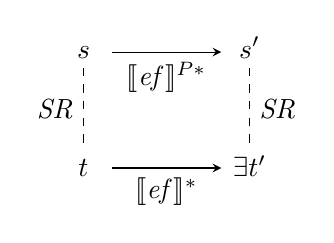
\begin{tikzpicture}
  \matrix (m) [matrix of math nodes,row sep=3em,column sep=4em,minimum width=2em]
  {
	  s & \vphantom{s}\smash{s'} \\
	 t & \vphantom{t}\smash{\exists t'} \\};
  \path[-stealth]
	(m-1-1) edge [dashed, -] node [left] {$\mathit{SR}$} (m-2-1)
			edge node [below] {$\llbracket \mathit{ef} \rrbracket^{P*}$} (m-1-2)
	(m-2-1) edge node [below] {$\llbracket \mathit{ef} \rrbracket^*$} (m-2-2)
	(m-1-2) edge [dashed, -] node [right] {$\mathit{SR}$} (m-2-2);
\end{tikzpicture}
	\end{figure}
\end{proof}

\section{Proof of theorem}

Similarly to lemmas, we separate the theorem into two parts, and alter it slightly to make it more consistent with what we have proved in Agda:

\begin{theorem}
\begin{multline*}
      \forall s, s', s'' \in \mathit{ProgState^\dagger} \ldotp\\\mathit{Init^P(s)} \land s \llbracket \mathit{(w \lor f)\ast} \cdot f \rrbracket^P s' \land s' \llbracket \mathit{w\ast} \cdot w^c \cdot \mathit{r^c\ast} \cdot r \rrbracket^P s'' \\ \implies \mathit{read(s')} \equiv \mathit{read(s'')}
\end{multline*}
\end{theorem}
\begin{proof}
	From $\mathit{initialisation}$ and repetively applying \cref{lemma-1} to the first relation, we have $\mathit{AR(s, t)}$ and $\mathit{AR(s', t')}$.
	The theorem can then be sketched as follows:
	\begin{figure} [h] \centering
		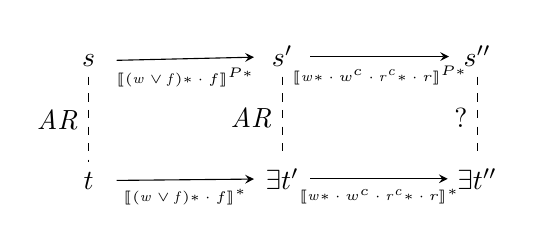
\begin{tikzpicture}
			\matrix (m) [matrix of math nodes, row sep=3em, column sep=5em, minimum width=2em]
			{ s & s' & s'' \\
			  t & \exists t' & \exists t'' \\};
			\path[-stealth]
			(m-1-1) edge [dashed, -] node [left] {$\mathit{AR}$} (m-2-1)
					edge node [below] {\tiny{$\llbracket \mathit{(w \lor f)*} \cdot f \rrbracket^{P*}$}} (m-1-2)
			(m-2-1) edge node [below] {\tiny{$\llbracket \mathit{(w \lor f)*} \cdot f \rrbracket^*$}} (m-2-2)
			(m-1-2) edge [dashed, -] node [left] {$\mathit{AR}$} (m-2-2)
					edge node [below] {\tiny{$\llbracket \mathit{w*} \cdot w^c \cdot \mathit{r^c*} \cdot r \rrbracket^{P*}$}} (m-1-3)
			(m-2-2) edge node [below] {\tiny{$\llbracket \mathit{w*} \cdot w^c \cdot \mathit{r^c*} \cdot r \rrbracket^*$}} (m-2-3)
			(m-1-3) edge [dashed, -] node [left] {?} (m-2-3);

		\end{tikzpicture}
	\end{figure}\\
	We can find some intermidiate states $s'_1$, $s'_2$, $s'_3$, and by applying \cref{lemma-1} repetively to obtain
	\begin{figure} [h] \centering
		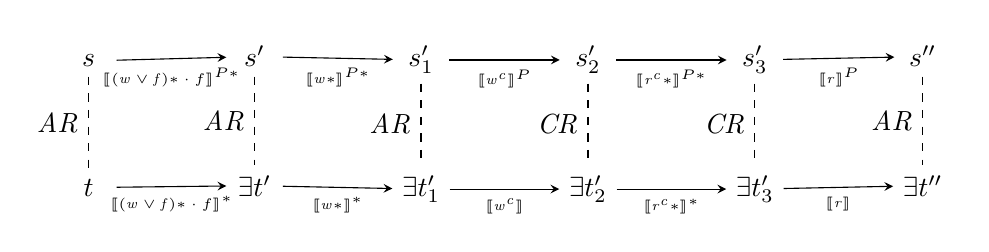
\begin{tikzpicture}
			\matrix (m) [matrix of math nodes, row sep=3em, column sep=4em, minimum width=2em]
			{ s & s' & s'_1 & s'_2 & s'_3 & s'' \\
			  t & \exists t' & \exists t'_1 & \exists t'_2 & \exists t'_3 & \exists t'' \\};
			\path[-stealth]
			(m-1-1) edge [dashed, -] node [left] {$\mathit{AR}$} (m-2-1)
					edge node [below] {\tiny{$\llbracket \mathit{(w \lor f)*} \cdot f \rrbracket^{P*}$}} (m-1-2)
			(m-2-1) edge node [below] {\tiny{$\llbracket \mathit{(w \lor f)*} \cdot f \rrbracket^*$}} (m-2-2)
			(m-1-2) edge [dashed, -] node [left] {$\mathit{AR}$} (m-2-2)
					edge node [below] {\tiny{$\llbracket \mathit{w*}  \rrbracket^{P*}$}} (m-1-3)
			(m-2-2) edge node [below] {\tiny{$\llbracket \mathit{w*} \rrbracket^*$}} (m-2-3)
			(m-1-3) edge [dashed, -] node [left] {$\mathit{AR}$} (m-2-3)
					edge node [below] {\tiny{$\llbracket \mathit{w^c}  \rrbracket^{P}$}} (m-1-4)
			(m-2-3) edge node [below] {\tiny{$\llbracket \mathit{w^c} \rrbracket$}} (m-2-4)
			(m-1-4) edge [dashed, -] node [left] {$\mathit{CR}$} (m-2-4)
					edge node [below] {\tiny{$\llbracket \mathit{r^c*}  \rrbracket^{P*}$}} (m-1-5)
			(m-2-4) edge node [below] {\tiny{$\llbracket \mathit{r^c*} \rrbracket^*$}} (m-2-5)
			(m-1-5) edge [dashed, -] node [left] {$\mathit{CR}$} (m-2-5)
					edge node [below] {\tiny{$\llbracket \mathit{r}  \rrbracket^{P}$}} (m-1-6)
			(m-2-5) edge node [below] {\tiny{$\llbracket \mathit{r} \rrbracket$}} (m-2-6)
			(m-1-6) edge [dashed, -] node [left] {$\mathit{AR}$} (m-2-6);

		\end{tikzpicture}
	\end{figure}\\
	thus complete the proof:
\begin{align*}
	\mathit{read(s)}   &\equiv \mathit{volatile(t)}   \tag{Observational Equivalence} \\
	& \qquad \quad \rotatebox{90}{$\equiv$} \tag{\cref{lemma-2-1}}\\
	\mathit{read(s'')} &\equiv \mathit{volatile(t'')} \tag{Observational Equivalence}
\end{align*} `
\end{proof}

\begin{theorem}
\begin{multline*}
      \forall s, s', s'', s''' \in \mathit{ProgState^\dagger} \ldotp\\\mathit{Init^P(s)} \land s \llbracket \mathit{(w \lor f)\ast} \cdot f \rrbracket^P s' \land
      s' \llbracket \mathit{w\ast} \rrbracket^P s'' \land
      s'' \llbracket f^c \cdot \mathit{r^c\ast} \cdot r \rrbracket^P s'''\\
      \implies \mathit{read(s')} \equiv \mathit{read(s''')} \lor \mathit{read(s'')} \equiv \mathit{read(s''')}
\end{multline*}
\end{theorem}


\end{document}
